\beginsong{Hier wächst kein Ahorn}[
    txt={Jooschen Engelke}, 
    mel={tejo (Walter Scherf)}, 
    jahr={1951}, 
    bo={182}, 
    siru={102},
]

\beginverse
\endverse
\centering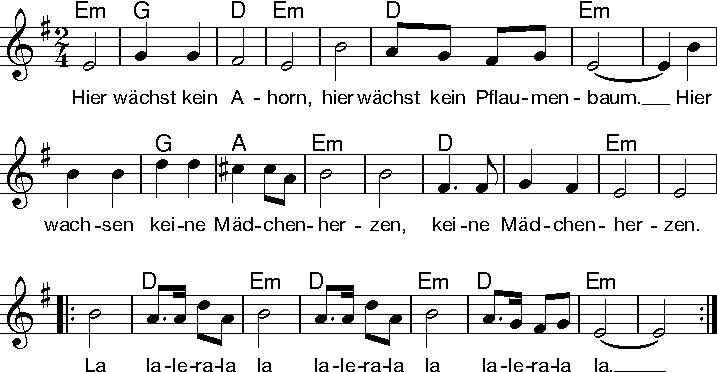
\includegraphics[width=1\textwidth]{Noten/Lied051.pdf}	


\beginverse
\[Em]Hier \[G]wächst der \[D]Thy\[Em]mian, hier \[D]wächst der Ginster\[Em]strauch
und Dornen \[G]wachsen \[A]aus den \[Em]Steinen, \[D]Dornen aus den \[Em]Steinen.
\endverse

\beginchorus
\lrep \[Em]La \[D]lalerala \[Em]la \[D]lalerala \[Em]la, \[D]lalerala \[Em]la. \rrep
\endchorus

\beginverse
^Hier ^wächst der ^Hand^schar, hier ^wächst der Flinten^lauf
und blüh'n wie ^Lilien ^blüh'n im ^Mondlicht, ^Lilien blüh'n im ^Mondlicht.
\endverse

\printchorus

\beginverse
^Und ^morgen ^A^bend und ^wenn der Nachtwind ^weht,
kommt unser ^Gene^ral ge^ritten, ^unser General ge^ritten.
\endverse

\printchorus

\beginverse
^Und ^bringt uns ^Ra^ki, hej ^ho bogami ^hej,
und bringt uns ^tausend ^Golddu^katen, ^tausend Golddu^katen.
\endverse

\printchorus

\endsong

\beginscripture{}
Das Lied ist angelehnt an ein Volkslied aus Montenegro.
\endscripture
